\documentclass[a4paper,12pt]{article}
\usepackage{fullpage}
\usepackage{hyperref}
\usepackage{url}
\usepackage{graphicx}
%\usepackage{polski}
\usepackage[utf8]{inputenc}

\setlength{\parindent}{0pt}
\addtolength{\parskip}{\baselineskip}

\title{3rd Year Group Project\\Report Three\\}

\author{
    \small{Rafał Szymański}\\
  	\and
    \small{Maciek Albin}\\
    \and
    \small{Sam Wong}\\
    \and  
    \small{Suhaib Sarmad}\\
		\and
		\small{Jamal Khan}\\
		\and
		\small{\{rs2909, mja108, sw2309, sss308, jzk09\}@doc.ic.ac.uk}
		\and
		\\Department of Computing - Imperial College London
}

\date{}

\begin{document} 
	\maketitle
	
	\section{Testing}
	
	  \subsection{Logging and Debugging}
	
	  Instead of using standard print statements to output the state of our system, which is composed of the RSS, Analysis and Twitter Thread, we incorporated a flexible event logging system.\\
	We are able to leave our system and if an error occurs we can trace exactly which thread caused it and at which point in the program as opposed to the usual debugging.
  The logger was also incorporated so that we have different levels of importance in logging i.e. have logging for general information of what is going on in the system and logging for errors. We are also able to log messages to different output sinks including the console and files.
	
	  \begin{figure}[ht!]
				  \centering
					  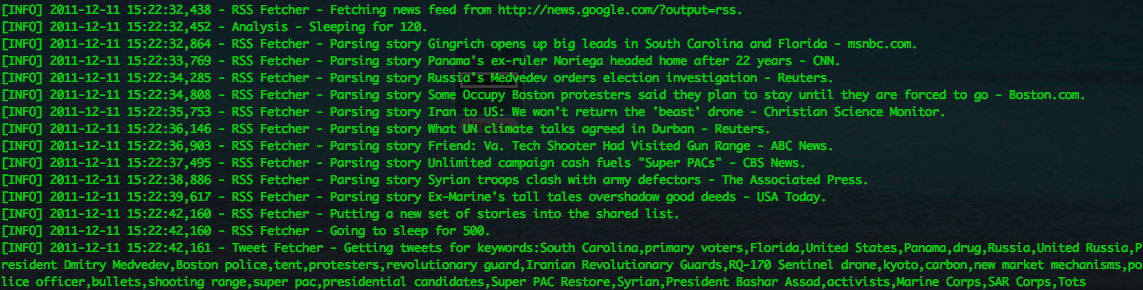
\includegraphics[scale=0.4]{logger.png}
				    \caption{Customised Logger}
	  \end{figure}
	
	  \subsection{Unit Testing}
	
	For testing various parts of the system we used unit tests to check that the code we were writing did not brake existing functionality that we already had.
	
	\section{General Validation}
	
	\section{Managerial Documentation}
	
		\subsection{Collaboration Tools Used}
		
			\subsubsection{Git}
			
			We have used the git version control system for keeping track of the project, for easily reverting if there is a problem, and for having a very quick deploy mechanism. Whenever a code push occurs to our git repository, we have a git post-receive hook that copies the static files appropriately, and restarts the appropriate processes. This means that as soon as a code push occurs, the new version is live.
			
			\subsubsection{Trello}
			
			Trello\footnote{\url{http://trello.com}} is a very good piece of software by FogCreek. It is a digital board that allows you to create post-its and write the product backlog, and move tasks between the product backlog, the current iteration, and the finished tasks. We plan to extract and append the Trello history to our final report, to show progress. Here is a screenshot of how Trello works:
			
			\begin{figure}[ht!]
						\centering
							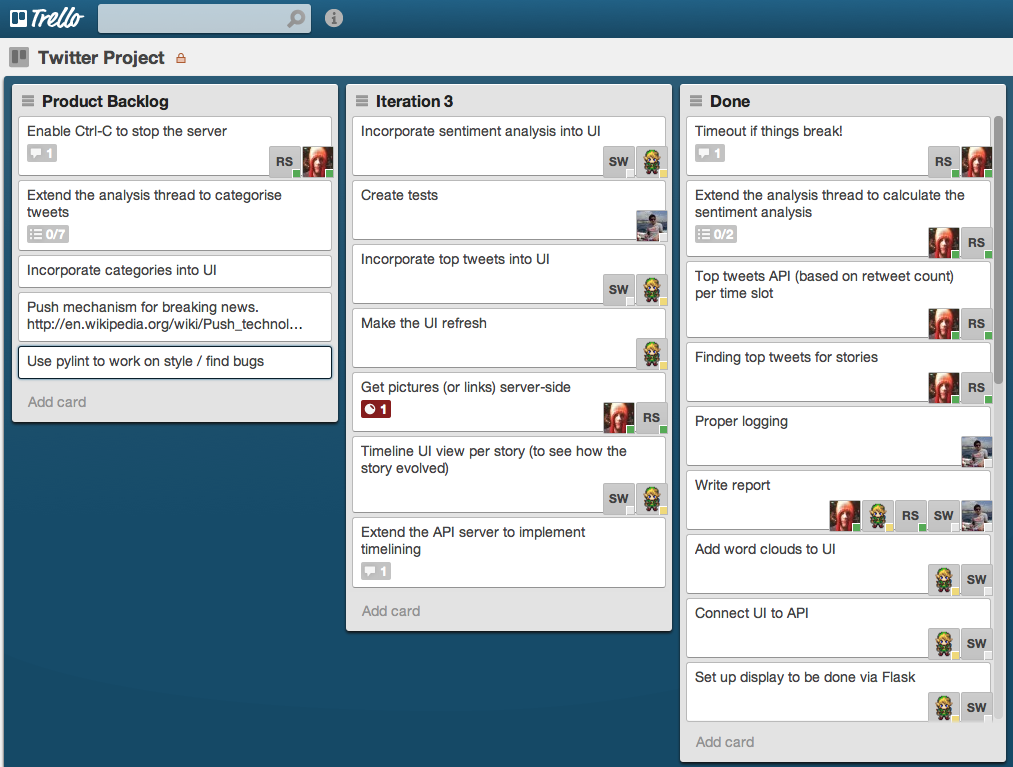
\includegraphics[scale=0.4]{trello1.png}
						\caption{Trello project management board}
			\end{figure}

		
		\subsection{Management policies}
		
		\subsection{Management of knowledge transfer within the group}
	
  

\end{document}
